
\documentclass[11pt,a4paper,oneside]{report}

% ============================================================
% Shader Alchemist
% Research Proposal / System Design / Technical Documentation
% ============================================================

\usepackage[a4paper,margin=1in,headheight=15pt]{geometry}
\usepackage[T1]{fontenc}
\usepackage[utf8]{inputenc}
\usepackage{lmodern}
\usepackage{microtype}
\usepackage{amsmath,amssymb,mathtools}
\usepackage{booktabs,longtable,array,tabularx,multirow}
\usepackage{graphicx}
\usepackage{xcolor}
\usepackage{tikz}
\usetikzlibrary{
  arrows.meta,
  positioning,
  shapes.geometric,
  shapes.multipart,
  fit,
  calc,
  backgrounds,
  matrix,
  decorations.pathreplacing
}
\usepackage{pgfgantt}
\usepackage{listings}
\usepackage{enumitem}
\usepackage{hyperref}
\usepackage{cleveref}
\usepackage{fancyhdr}
\usepackage{float}
\usepackage{caption}
\usepackage{subcaption}
\usepackage{siunitx}
\usepackage{algorithm}
\usepackage{algpseudocode}
\usepackage{url}
\usepackage{bookmark}

\hypersetup{
  colorlinks=true,
  linkcolor=blue!50!black,
  citecolor=green!40!black,
  urlcolor=blue!60!black,
  pdftitle={Shader Alchemist},
  pdfauthor={Shader Alchemist Research Project}
}

\pagestyle{fancy}
\fancyhf{}
\fancyhead[L]{Shader Alchemist}
\fancyhead[R]{System Design and Research Proposal}
\fancyfoot[C]{\thepage}

\definecolor{codebg}{RGB}{245,247,250}
\definecolor{codeframe}{RGB}{180,185,195}
\definecolor{architect}{RGB}{220,235,250}
\definecolor{writer}{RGB}{230,245,225}
\definecolor{evaluator}{RGB}{250,235,215}
\definecolor{infra}{RGB}{235,230,250}
\definecolor{risk}{RGB}{250,225,225}

\lstdefinelanguage{WGSL}{
  morekeywords={
    struct,var,let,fn,return,if,else,for,loop,
    array,vec2,vec3,vec4,f32,i32,u32,bool,
    compute,workgroup,storage,uniform,read,read_write,
    group,binding,location,builtin,global_invocation_id,
    workgroup_id,local_invocation_id,workgroup_size
  },
  sensitive=true,
  morecomment=[l]{//},
  morestring=[b]"
}
\lstset{
  backgroundcolor=\color{codebg},
  frame=single,
  rulecolor=\color{codeframe},
  basicstyle=\ttfamily\small,
  columns=fullflexible,
  keepspaces=true,
  breaklines=true,
  showstringspaces=false
}

\newcommand{\SA}{\textsc{Shader Alchemist}}
\newcommand{\WGSL}{\textsc{WGSL}}
\newcommand{\WebGPU}{\textsc{WebGPU}}
\newcommand{\MathSpec}{\textsc{MathSpec}}
\newcommand{\ShaderArtifact}{\textsc{ShaderArtifact}}
\newcommand{\EvalReport}{\textsc{EvalReport}}
\newcommand{\SAState}{\textsc{ShaderAlchemistState}}

\title{
  \Huge\bfseries Shader Alchemist\\[0.4em]
  \Large An Agentic Compiler and Performance Engineering System\\
  for Verified and Optimized WebGPU Compute Shaders
}
\author{
  Research Proposal, System Architecture,\\
  Mathematical Specification, Evaluation Methodology,\\
  and Technical Documentation
}
\date{October 2026}

\begin{document}

\maketitle
\thispagestyle{empty}

\begin{abstract}
Modern GPU programming sits at an unusual intersection of mathematics, compiler construction,
parallel algorithms, hardware architecture, memory models, and empirical performance engineering.
Writing a correct compute shader is already difficult; writing one that is portable, safe,
measurably efficient, and appropriately tuned to a target WebGPU implementation is substantially
harder.

This document proposes \SA, an agentic shader engineering environment that converts a high-level
algorithmic or visual requirement into a formally structured mathematical specification, a
candidate \WGSL compute pipeline, and an empirically evaluated implementation. The central design
principle is separation of concerns: a \emph{Math Architect} establishes mathematical and parallel
execution invariants; a \emph{WGSL Writer} realizes those invariants as shader code; and a
\emph{Performance Evaluator} executes the artifact inside an isolated WebGPU harness, observes
validation and timing information, and returns structured evidence to an iterative refinement loop.

The proposed system is deliberately more than an LLM code generator. Its core object is a
closed-loop engineering process:
\[
\text{intent}\rightarrow\text{formal specification}\rightarrow
\text{shader artifact}\rightarrow\text{measurement}\rightarrow
\text{diagnosis}\rightarrow\text{refinement}.
\]
The architecture therefore treats generated shader source as an intermediate artifact rather
than as the final truth. Correctness is established through static constraints, WebGPU validation,
differential tests, numerical invariants, and controlled execution. Performance is treated as an
empirical property of a specific workload and execution environment, not as a claim inferred from
source code alone.

The proposal further introduces hardware capability profiles, multi-objective optimization,
counterfactual optimization experiments, reproducible benchmark suites, deterministic replay,
security isolation, compiler-backed validation, and future support for subgroup operations,
\texttt{shader-f16}, specialization, autotuning, cross-backend compilation, and learned performance
models. The result is intended as a research platform as much as a developer tool: a system in
which agentic reasoning and GPU measurement can be studied as a unified optimization process.
\end{abstract}

\begingroup
\small
\tableofcontents
\endgroup
\listoffigures

\chapter{Introduction}

\section{Motivation}

GPU programming traditionally assumes that the programmer understands several layers of the
machine simultaneously. At the algorithmic level, one must understand the mathematical operation.
At the parallel level, one must decide how independent work is mapped onto invocations and
workgroups. At the memory level, one must understand buffer layouts, alignment, access modes,
locality, synchronization, and hazards. At the API level, one must construct pipelines, bind
resources, select supported features, and respect validation rules. Finally, at the hardware level,
one must reason about occupancy, memory bandwidth, instruction throughput, divergence, cache
behavior, and the particular architecture of the target GPU.

A language model can produce shader source quickly, but source generation alone does not solve this
problem. A shader can be syntactically plausible and mathematically coherent while still being
incorrect because of a binding mismatch, an invalid resource usage, a race condition, a wrong
dispatch geometry, an incompatible feature assumption, or a host/shader memory-layout mismatch.
It can also be correct yet substantially slower than an alternative implementation.

\SA is therefore designed around a stronger abstraction:

\begin{quote}
\emph{A generated shader is a hypothesis about an implementation. The execution harness supplies
evidence about whether that hypothesis is correct and how well it performs.}
\end{quote}

This transforms shader generation from a one-shot synthesis task into an experimental engineering
loop.

\section{Problem Statement}

Given a high-level request $R$, a target workload $W$, a hardware capability profile $H$, and a
performance objective $B$, the system seeks a shader pipeline $P$ satisfying:

\begin{align}
P &\models C_{\mathrm{syntax}},\\
P &\models C_{\mathrm{layout}},\\
P &\models C_{\mathrm{resource}},\\
P &\models C_{\mathrm{memory}},\\
P &\models C_{\mathrm{numerical}},\\
P &\models C_{\mathrm{semantic}},
\end{align}

while minimizing a performance objective such as

\begin{equation}
J(P)=
\lambda_t T(P)+
\lambda_m M(P)+
\lambda_e E(P)+
\lambda_r R_{\mathrm{risk}}(P),
\end{equation}

subject to

\begin{equation}
T(P)\le B_t,
\qquad
M(P)\le B_m,
\qquad
R_{\mathrm{risk}}(P)\le B_r.
\end{equation}

Here $T$ is measured execution latency, $M$ is a memory-related cost,
$E$ may represent energy or estimated energy cost when available, and
$R_{\mathrm{risk}}$ summarizes execution and portability risk.

The important point is that the optimization target is not ``shorter code'' or ``more elegant
WGSL.'' It is a constrained system-level objective.

\section{Research Questions}

The proposed platform enables investigation of several research questions:

\begin{enumerate}[label=\textbf{RQ\arabic*:}]
  \item Can decomposition into mathematical planning, shader synthesis, and empirical evaluation
        reduce the rate of shader correctness failures compared with direct generation?
  \item Can an agent use measured GPU feedback to discover optimizations that are difficult to
        infer reliably from source inspection alone?
  \item How should shader optimization balance latency, memory footprint, portability, numerical
        accuracy, and implementation complexity?
  \item Can hardware capability profiles allow a generated shader to adapt to heterogeneous
        WebGPU implementations without sacrificing correctness?
  \item How much optimization can be automated before the search space becomes computationally
        prohibitive?
  \item Can historical benchmark data become a learned prior for selecting promising optimization
        transformations?
\end{enumerate}

\section{Scope}

The initial system focuses on compute-oriented \WebGPU{} workloads and \WGSL{} shader generation.
Examples include:

\begin{itemize}
  \item spatial hashing and particle binning,
  \item particle and fluid simulation,
  \item image and tensor kernels,
  \item matrix and vector operations,
  \item reductions and prefix-style operations,
  \item cellular and grid simulations,
  \item procedural generation,
  \item image-processing kernels,
  \item broad-phase collision structures,
  \item graph and neighborhood computations.
\end{itemize}

The system is not initially intended to replace a general-purpose compiler, a full GPU profiler,
or a formal theorem prover. Instead, it composes these capabilities into an agentic engineering
workflow.

\subsection{Request and Support Contract}

Each workload should state its operation, input and output domains, element counts or grid
dimensions, data types, numerical tolerances, required features, and any memory or latency budget.
Separating hard constraints from preferences lets the optimizer reject an invalid candidate before
ranking its speed. A useful evaluation manifest also includes representative workload sizes rather
than a single convenient input, so the system can distinguish a consistently useful optimization
from one that only benefits a narrow case.

The initial scope is compute pipelines and their host-side execution contracts. Rendering,
real-time presentation, and graphics-pipeline optimization remain separate concerns; a generated
demo may visualize results, but visual similarity does not replace numerical and invariant-based
correctness checks.

\chapter{Design Principles}

\section{Principle 1: Specification Before Synthesis}

The first agent does not write shader code. It constructs a machine-checkable description of the
problem. This reduces ambiguity and gives later stages a stable contract.

The transformation is

\[
R \longrightarrow \mathcal{M},
\]

where $R$ is natural-language intent and $\mathcal{M}$ is a \MathSpec{} containing:

\begin{equation}
\mathcal{M} =
\{
\mathcal{A},
\mathcal{D},
\mathcal{L},
\mathcal{B},
\mathcal{S},
\mathcal{N},
\mathcal{H},
\mathcal{V}
\}.
\end{equation}

The components denote algorithmic semantics, domain decomposition, layout, bindings, synchronization,
numerical constraints, hardware requirements, and verification obligations.

\section{Principle 2: Source Is Not Evidence}

The system must distinguish between:

\begin{itemize}
  \item \emph{syntactic validity},
  \item \emph{API validation},
  \item \emph{memory safety},
  \item \emph{semantic correctness},
  \item \emph{numerical accuracy},
  \item \emph{performance}.
\end{itemize}

Passing one does not imply passing the others.

\section{Principle 3: Optimization Is Experimental}

An optimization transformation should ideally be represented as an experiment:

\[
P_i
\xrightarrow{\tau}
P_{i+1},
\]

where $\tau$ is a named transformation such as:

\begin{itemize}
  \item workgroup-size change,
  \item structure-of-arrays conversion,
  \item shared-memory tiling,
  \item branch restructuring,
  \item loop transformation,
  \item precision reduction,
  \item algorithmic decomposition,
  \item subgroup-based reduction,
  \item dispatch decomposition.
\end{itemize}

The evaluator compares $P_i$ and $P_{i+1}$ under the same benchmark conditions.

\section{Principle 4: Hardware Capability Is First-Class State}

WebGPU exposes optional capabilities. The system must not assume that a feature is universally
available. Instead, the capability profile is represented as:

\[
H =
\{
F,\ L,\ M,\ Q,\ P
\},
\]

where $F$ is the supported feature set, $L$ contains device limits, $M$ contains memory-related
properties, $Q$ contains query/timing capabilities, and $P$ contains platform metadata.

The optimization planner can then generate a capability-dependent strategy:

\[
\pi^\star = \arg\min_{\pi\in\Pi(H)}J(\pi).
\]

\chapter{System Architecture}

\section{Top-Level Architecture}

The architecture is a hybrid of sequential orchestration, iterative refinement, compiler-style
intermediate representations, and an external execution harness.

\begin{figure}[H]
\centering
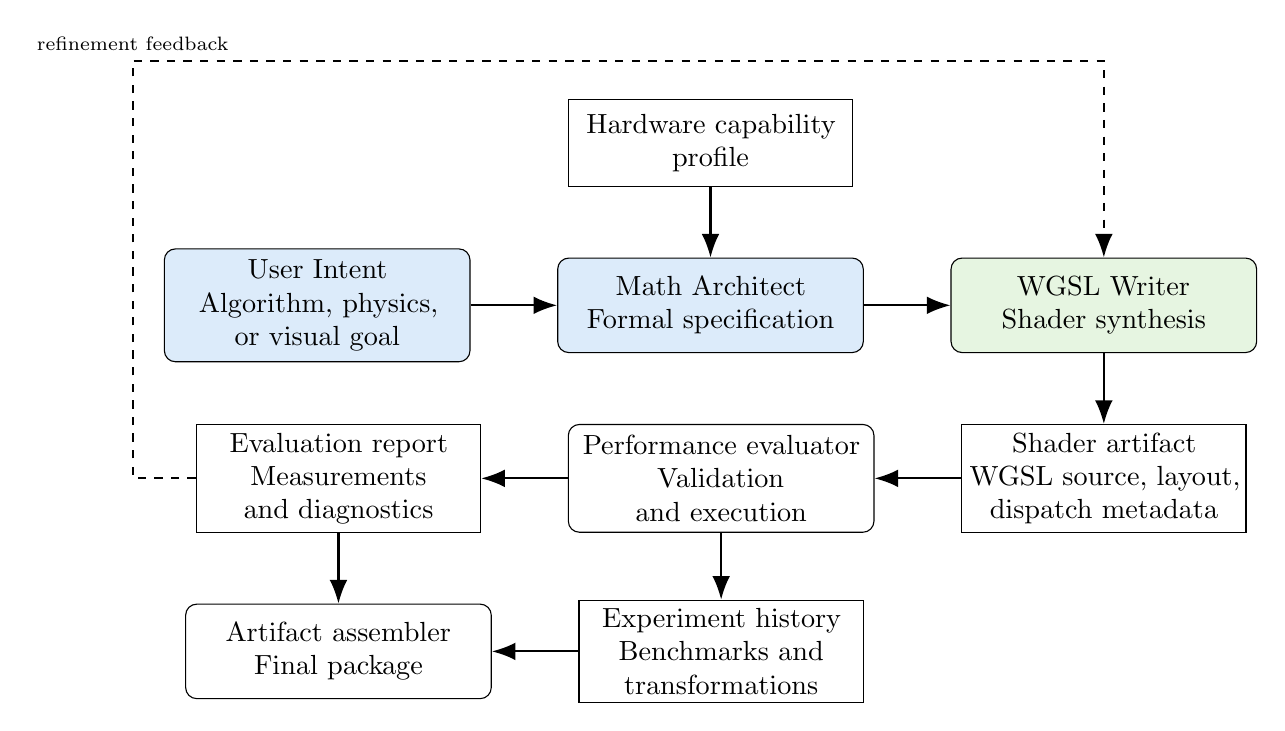
\begin{tikzpicture}[
  node distance=9mm and 11mm,
  stage/.style={rectangle,rounded corners,draw,align=center,text width=36mm,minimum height=12mm,inner sep=4pt},
  record/.style={rectangle,draw,align=center,text width=34mm,minimum height=11mm,inner sep=3pt},
  arrow/.style={-{Latex[length=3mm]},thick},
]
\node[stage,fill=architect] (user) {User Intent\\Algorithm, physics, or visual goal};
\node[stage,fill=architect,right=of user] (math) {Math Architect\\Formal specification};
\node[stage,fill=writer,right=of math] (writer) {WGSL Writer\\Shader synthesis};
\node[record,above=of math] (caps) {Hardware capability\\profile};
\node[record,below=of writer] (artifact) {Shader artifact\\WGSL source, layout,\\dispatch metadata};
\node[stage,left=of artifact] (eval) {Performance evaluator\\Validation and execution};
\node[record,left=of eval] (report) {Evaluation report\\Measurements and diagnostics};
\node[stage,below=of report] (assembler) {Artifact assembler\\Final package};
\node[record,right=of assembler] (history) {Experiment history\\Benchmarks and transformations};

\draw[arrow] (user) -- (math);
\draw[arrow] (caps) -- (math);
\draw[arrow] (math) -- (writer);
\draw[arrow] (writer) -- (artifact);
\draw[arrow] (artifact) -- (eval);
\draw[arrow] (eval) -- (report);
\draw[arrow,dashed] (report.west) -- ++(-8mm,0) |- node[pos=0.5,above,font=\scriptsize]{refinement feedback} ($(writer.north)+(0,25mm)$) -- (writer.north);
\draw[arrow] (report) -- (assembler);
\draw[arrow] (eval) -- (history);
\draw[arrow] (history) -- (assembler);
\end{tikzpicture}
\caption{High-level architecture of Shader Alchemist.}
\label{fig:topology}
\end{figure}

The system has five logical planes:

\begin{enumerate}
  \item \textbf{Intent plane}: natural-language and structured user requirements.
  \item \textbf{Reasoning plane}: mathematical specification and optimization reasoning.
  \item \textbf{Artifact plane}: WGSL, binding layouts, dispatch configuration, and host metadata.
  \item \textbf{Execution plane}: isolated WebGPU compilation and GPU execution.
  \item \textbf{Evidence plane}: measurements, validation logs, correctness results, and experiment history.
\end{enumerate}

\section{Agent Topology}

The principal agent topology is:

\[
\boxed{
\text{Math Architect}
\rightarrow
\left[
\text{WGSL Writer}
\rightarrow
\text{Performance Evaluator}
\right]^{k}
\rightarrow
\text{Assembler}
}
\]

where $k$ is bounded by the configured refinement budget.

A second-level supervisory agent can later be introduced:

\[
\text{Supervisor}
\rightarrow
\{\text{Math},\text{Codegen},\text{Evaluation},\text{Optimization}\}.
\]

This should be introduced only after the deterministic pipeline is stable. Otherwise the system
risks becoming an opaque collection of agents whose interactions are difficult to reproduce.

\section{Stage Contracts and Feedback Semantics}

The orchestrator should pass versioned structured artifacts between stages instead of relying on
unrecorded conversational context. The Math Architect owns the semantic contract and records its
assumptions. The WGSL Writer may choose a representation, data layout, or workgroup configuration,
but a change to the algorithm's meaning must be returned as a revised specification rather than
silently embedded in source code.

The evaluator returns a structured report that separates parsing, pipeline validation,
correctness, numerical error, and timing. The orchestrator accepts a candidate only when all hard
checks pass; otherwise it routes the failure to the responsible stage. A performance improvement
must be measured against the same input, reference, and device configuration as its baseline. This
keeps the feedback loop auditable and prevents an agent's explanation from being mistaken for
execution evidence.

\chapter{Formal Problem Model}

\section{Input Model}

A request is modeled as:

\begin{equation}
X = (R,W,H,O,C),
\end{equation}

where:

\begin{itemize}
  \item $R$ = semantic request,
  \item $W$ = workload specification,
  \item $H$ = hardware capability profile,
  \item $O$ = optimization objective,
  \item $C$ = correctness and safety constraints.
\end{itemize}

For example, a request for a 3D particle simulation might specify:

\[
N=10^6,\qquad
p_i\in\mathbb{R}^3,\qquad
v_i\in\mathbb{R}^3,
\]

with cell width $s$ and spatial domain $\Omega$.

\section{Parallel Decomposition}

Suppose the problem contains $N$ independent particles and the shader uses a one-dimensional
workgroup of width $W$.

The global invocation index is

\begin{equation}
g = Wg_w+\ell,
\end{equation}

where $g_w$ is the workgroup index and $\ell$ is the local invocation index.

The number of workgroups is

\begin{equation}
G=\left\lceil\frac{N}{W}\right\rceil.
\end{equation}

The valid domain condition is

\begin{equation}
0\le g<N.
\end{equation}

For a three-dimensional domain, let $\mathbf{N}$ denote the dimensions and $\mathbf{W}$ the
workgroup shape:

\[
\mathbf{N}=(N_x,N_y,N_z),
\qquad
\mathbf{W}=(W_x,W_y,W_z).
\]

\begin{align}
G_x &= \left\lceil\frac{N_x}{W_x}\right\rceil,\\
G_y &= \left\lceil\frac{N_y}{W_y}\right\rceil,\\
G_z &= \left\lceil\frac{N_z}{W_z}\right\rceil.
\end{align}

The dispatch geometry is therefore derived from the problem domain rather than selected
independently by the code generator.

The rounded dispatch launches $GW$ invocations, of which only $N$ are useful. A simple measure
of lane utilization for this one-dimensional mapping is

\begin{equation}
\eta_{\mathrm{dispatch}}=\frac{N}{GW},
\qquad N>0,\quad 0<\eta_{\mathrm{dispatch}}\le 1.
\end{equation}

This ratio describes tail waste, not hardware occupancy. The final partial workgroup must still
use a bounds check; dispatch rounding never licenses an out-of-domain memory access. When a
three-dimensional launch is mapped onto a flattened array, coordinates $(x,y,z)$ can be mapped
to a linear element index by

\begin{equation}
i=x+N_x(y+N_yz),
\qquad 0\le i<N_xN_yN_z.
\end{equation}

The inverse mapping is useful when an algorithm needs coordinates after loading a linear index.
All products used to form dispatch sizes or byte offsets must be checked against the host integer
range and device limits before buffers are allocated.

\section{Spatial Hashing Example}

For a particle position

\[
\mathbf{p}=(x,y,z),
\]

and cell size $s$, with domain origin $\mathbf{o}$, define

\begin{equation}
\mathbf{c}=
\left\lfloor
\frac{\mathbf{p}-\mathbf{o}}{s}
\right\rfloor.
\end{equation}

A hash function may be constructed as

\begin{equation}
h(\mathbf{c})
=
\left(
c_xP_x
\oplus
c_yP_y
\oplus
c_zP_z
\right)
\bmod B,
\end{equation}

where $P_x,P_y,P_z$ are selected integer constants and $B$ is the number of hash-table buckets.

The cell coordinate is the semantic key; the bucket index is only an acceleration structure.
Different cells may map to the same bucket, so a correct lookup must retain or reconstruct the
full cell key and filter candidates by cell equality. Under independent uniform hashing, the
expected number of pairs among $N$ distinct keys that share a bucket is

\begin{equation}
\mathbb{E}[C]=\binom{N}{2}\frac{1}{B}
=\frac{N(N-1)}{2B}.
\end{equation}

Here $N$ counts distinct keys, not particles that intentionally occupy the same cell. For a
fixed-capacity bucket of size $K$, an idealized independent-uniform model gives the per-bucket
overflow probability for $N$ independently inserted entries:

\begin{equation}
\Pr[X>K]
=\sum_{k=K+1}^{N}\binom{N}{k}
\left(\frac{1}{B}\right)^k
\left(1-\frac{1}{B}\right)^{N-k},
\qquad X\sim\operatorname{Binomial}\left(N,\frac{1}{B}\right).
\end{equation}

This estimate is a sizing aid rather than a correctness proof: real particle distributions can be
highly nonuniform. The implementation must define overflow behavior explicitly, for example by
using a linked overflow structure, a retry pass, or a capacity error reported to the host. Hash
arithmetic must also specify how signed coordinates are converted to unsigned bit patterns and how
the final remainder is made nonnegative; host-language signed remainder conventions must not be
assumed to match shader arithmetic.

The system must additionally reason about:

\begin{itemize}
  \item signed versus unsigned integer conversion,
  \item negative spatial coordinates,
  \item hash collisions,
  \item bucket capacity,
  \item atomicity of concurrent insertion,
  \item overflow behavior,
  \item deterministic ordering requirements.
\end{itemize}

This is a crucial distinction: a mathematically valid hash function does not automatically
produce a correct parallel spatial index.

\section{Work and Memory Cost Model}

Static operation counts help identify plausible bottlenecks, but they do not replace GPU timing.
Let $F$ be the number of arithmetic operations executed by a workload and $Q$ the number of bytes
transferred between device memory and the compute units. Its arithmetic intensity is

\begin{equation}
I=\frac{F}{Q}
\quad\text{operations per byte}.
\end{equation}

Under an idealized roofline model with peak arithmetic throughput $\Pi_{\max}$ and memory
bandwidth $\beta_{\max}$, execution time has the lower bound

\begin{equation}
T\ge \max\left(\frac{F}{\Pi_{\max}},\frac{Q}{\beta_{\max}}\right).
\end{equation}

This bound omits launch overhead, synchronization, cache effects, occupancy limits, and contention;
the evaluator therefore uses it to form hypotheses, not to predict a guaranteed runtime. For a
multi-pass pipeline with $m$ passes, a more complete first-order model is

\begin{equation}
T_{\mathrm{pipeline}}\approx
\sum_{j=1}^{m}T_j+(m-1)T_{\mathrm{boundary}},
\end{equation}

where $T_{\mathrm{boundary}}$ represents inter-pass command and synchronization overhead. This
explains why eliminating an intermediate buffer or pass can matter even when each individual
kernel is already bandwidth-efficient.

\chapter{Mathematical Architect}

\section{Role}

The Math Architect converts natural-language intent into an explicit mathematical and execution
contract. Its output should be sufficiently precise that a compiler engineer could implement the
algorithm without needing to reinterpret the original prompt.

\section{Responsibilities}

The agent determines:

\begin{enumerate}
  \item mathematical equations;
  \item input/output domains;
  \item data dependencies;
  \item parallel decomposition;
  \item workgroup shape candidates;
  \item dispatch bounds;
  \item buffer layouts;
  \item synchronization requirements;
  \item atomic operations;
  \item numerical precision;
  \item invariants;
  \item reference implementation semantics;
  \item correctness tests.
\end{enumerate}

\section{Dependency Graph}

For a multi-stage computation, the architect creates a directed acyclic graph where possible:

\begin{figure}[H]
\centering
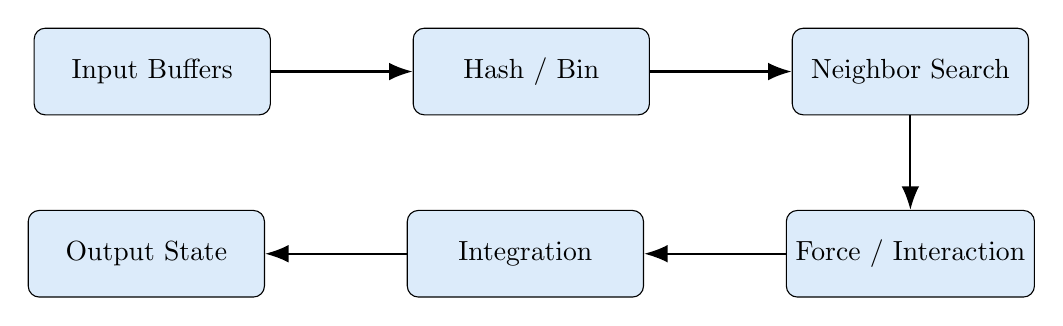
\begin{tikzpicture}[
  node distance=12mm and 18mm,
  op/.style={rectangle,rounded corners,draw,fill=architect,minimum width=30mm,minimum height=11mm,align=center},
  arr/.style={-{Latex[length=3mm]},thick}
]
\node[op] (input) {Input Buffers};
\node[op,right=of input] (hash) {Hash / Bin};
\node[op,right=of hash] (neighbors) {Neighbor Search};
\node[op,below=of neighbors] (forces) {Force / Interaction};
\node[op,left=of forces] (integrate) {Integration};
\node[op,left=of integrate] (output) {Output State};
\draw[arr] (input)--(hash);
\draw[arr] (hash)--(neighbors);
\draw[arr] (neighbors)--(forces);
\draw[arr] (forces)--(integrate);
\draw[arr] (integrate)--(output);
\end{tikzpicture}
\caption{Example dependency graph for a particle simulation.}
\end{figure}

This graph becomes a scheduling problem:

\[
\mathcal{G}=(V,E),
\]

where $V$ contains computational stages and $E$ represents data dependencies.

A single dispatch is permitted only when all dependencies within the dispatch can be satisfied
without requiring unsupported cross-workgroup synchronization. Otherwise, the architect should
propose multiple passes.

\section{Layout Reasoning}

The architect must compute:

\begin{equation}
\mathrm{offset}(f_i)
=
\operatorname{roundUp}
\left(
\mathrm{offset}(f_{i-1})+\mathrm{size}(f_{i-1}),
\mathrm{align}(f_i)
\right).
\end{equation}

For an array:

\begin{equation}
\mathrm{stride}(T)
=
\operatorname{roundUp}
\left(
\mathrm{size}(T),
\mathrm{align}(T)
\right),
\end{equation}

subject to the applicable address-space layout constraints.

The critical architectural rule is that \SA{} should not encode a universal ``16-byte padding''
heuristic. It should calculate the layout according to the actual WGSL type and the applicable
address space. For example, a \texttt{vec3<f32>} has 16-byte alignment, while its value size is
12 bytes; array stride and structure-member placement therefore require explicit layout reasoning.

For the following illustrative structure, the second vector cannot begin immediately after the
12-byte value of the first vector:

\begin{lstlisting}[language=WGSL,caption={WGSL record whose padding affects host-side serialization.}]
struct Particle {
  position : vec3<f32>,
  velocity : vec3<f32>,
};
\end{lstlisting}

The corresponding storage-buffer layout is:

\begin{center}
\begin{tabular}{lrrrr}
\toprule
\textbf{Member} & \textbf{Offset} & \textbf{Alignment} & \textbf{Value size} & \textbf{Next offset}\\
\midrule
\texttt{position} & 0 & 16 & 12 & 16\\
\texttt{velocity} & 16 & 16 & 12 & 32\\
\bottomrule
\end{tabular}
\end{center}

The structure alignment is 16 bytes and its array stride is 32 bytes. Host code must serialize
records using these offsets and strides, or deliberately choose a different representation such
as separate position and velocity arrays. The schema should record both the logical fields and
the concrete byte layout so that a host-side change cannot silently invalidate the shader.

\section{Synchronization Analysis}

Synchronization is modeled as a graph problem.

If invocation $a$ writes a memory location read by invocation $b$, then:

\[
a \prec_{\mathrm{write}} b
\]

must be enforced by a valid synchronization mechanism or by restructuring the algorithm so that
the accesses no longer race.

The architect distinguishes:

\begin{itemize}
  \item intra-invocation ordering,
  \item workgroup synchronization,
  \item storage-memory visibility,
  \item atomic read-modify-write operations,
  \item inter-dispatch ordering.
\end{itemize}

The architecture explicitly avoids assuming that a barrier magically synchronizes arbitrary
workgroups. When a dependency crosses workgroup boundaries, a multi-pass algorithm or another
valid synchronization strategy may be required.

\chapter{WGSL Writer}

\section{Role}

The WGSL Writer realizes the \MathSpec{} as a candidate shader artifact.

Its objective is not merely to produce syntactically valid WGSL. It must preserve the semantic
contract produced by the Math Architect.

\section{Transformation Pipeline}

The conceptual transformation is:

\[
\MathSpec
\xrightarrow{\text{lowering}}
\text{Shader IR}
\xrightarrow{\text{WGSL emission}}
\WGSL.
\]

A future implementation should introduce an intermediate representation rather than generating
WGSL directly from natural language.

\begin{figure}[H]
\centering
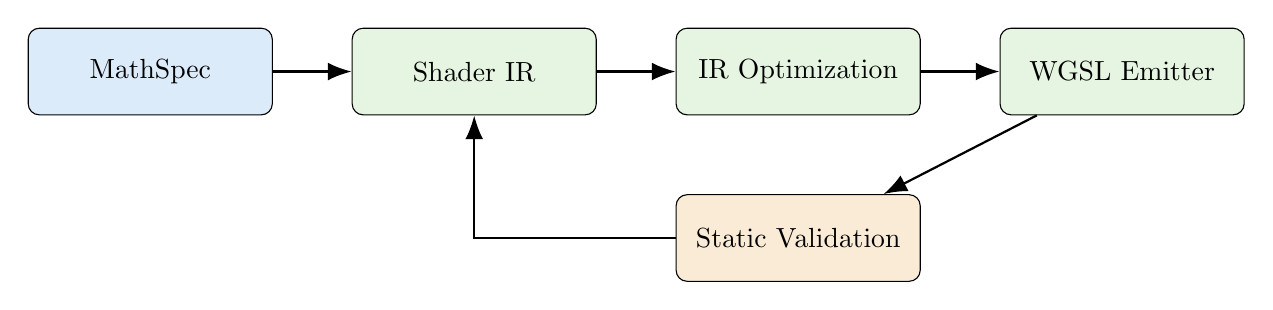
\begin{tikzpicture}[
  n/.style={rectangle,rounded corners,draw,minimum width=31mm,minimum height=11mm,align=center},
  a/.style={-{Latex[length=3mm]},thick}
]
\node[n,fill=architect] (m) {MathSpec};
\node[n,fill=writer,right=of m] (ir) {Shader IR};
\node[n,fill=writer,right=of ir] (opt) {IR Optimization};
\node[n,fill=writer,right=of opt] (emit) {WGSL Emitter};
\node[n,fill=evaluator,below=of opt] (lint) {Static Validation};
\draw[a] (m)--(ir);
\draw[a] (ir)--(opt);
\draw[a] (opt)--(emit);
\draw[a] (emit)--(lint);
\draw[a] (lint)-|(ir);
\end{tikzpicture}
\caption{Recommended compiler-style internal representation for shader synthesis.}
\end{figure}

\section{Shader IR}

The proposed IR should represent:

\begin{itemize}
  \item types,
  \item address spaces,
  \item resources,
  \item functions,
  \item loops,
  \item control flow,
  \item memory accesses,
  \item barriers,
  \item atomics,
  \item workgroup dimensions,
  \item numerical precision,
  \item transformation provenance.
\end{itemize}

An optimization can then operate on the IR without requiring the language model to regenerate
the entire shader from scratch.

\section{Worked Bounds-Safe Shader Example}

The following elementwise vector-add kernel demonstrates the connection between a \MathSpec{},
the WGSL resource contract, and dispatch geometry. It is intentionally small enough to serve as a
compiler and harness smoke test while still exercising storage bindings and a rounded dispatch.

\begin{lstlisting}[language=WGSL,caption={Bounds-safe vector addition using runtime-sized storage arrays.}]
struct FloatBuffer {
  values : array<f32>,
};

@group(0) @binding(0)
var<storage, read> lhs : FloatBuffer;

@group(0) @binding(1)
var<storage, read> rhs : FloatBuffer;

@group(0) @binding(2)
var<storage, read_write> output_buffer : FloatBuffer;

@compute @workgroup_size(64)
fn vector_add(@builtin(global_invocation_id) gid : vec3<u32>) {
  let index = gid.x;
  let output_length = arrayLength(&output_buffer.values);
  if (index >= output_length) {
    return;
  }
  if (index >= arrayLength(&lhs.values) || index >= arrayLength(&rhs.values)) {
    return;
  }
  output_buffer.values[index] = lhs.values[index] + rhs.values[index];
}
\end{lstlisting}

The host contract requires three storage buffers with compatible \texttt{f32} element layouts,
equal logical input lengths, and an output buffer of the same length. The per-invocation checks
prevent out-of-bounds accesses even if dispatch rounding creates extra invocations; host-side
validation remains responsible for rejecting inconsistent buffer lengths rather than treating a
partial output as successful. With $N$ elements and workgroup width $W=64$, the host dispatches
$\lceil N/64\rceil$ workgroups when $N>0$.

\begin{lstlisting}[caption={Host-side dispatch rule corresponding to the shader above.}]
const workgroupSize = 64;
if (elementCount > 0) {
  pass.dispatchWorkgroups(Math.ceil(elementCount / workgroupSize));
}
\end{lstlisting}

For $N=1025$, the dispatch contains 17 workgroups and 1088 invocations, so the final 63
invocations return without accessing memory. This example does not claim that a workgroup size of
64 is optimal; it provides a deterministic baseline against which candidate sizes can be tested.

\chapter{Performance Evaluator}

\section{Purpose}

The Performance Evaluator is the empirical core of the system. It answers questions that cannot
be established reliably from static reasoning alone:

\begin{itemize}
  \item Does the shader compile?
  \item Does the pipeline satisfy WebGPU validation?
  \item Does the workload produce the expected result?
  \item Does it remain within the memory and dispatch limits?
  \item How long does the compute pass take?
  \item Does the candidate improve upon the baseline?
\end{itemize}

\section{Execution Harness}

The proposed harness is isolated from the agent process.

\begin{figure}[H]
\centering
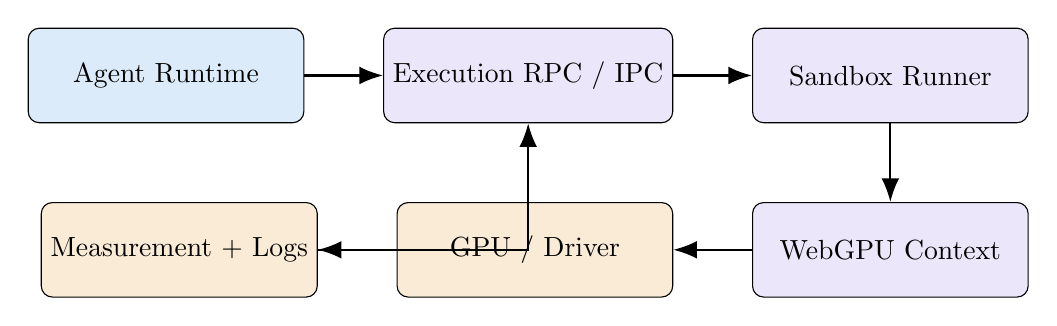
\begin{tikzpicture}[
  n/.style={rectangle,rounded corners,draw,minimum width=35mm,minimum height=12mm,align=center},
  a/.style={-{Latex[length=3mm]},thick}
]
\node[n,fill=architect] (agent) {Agent Runtime};
\node[n,fill=infra,right=of agent] (ipc) {Execution RPC / IPC};
\node[n,fill=infra,right=of ipc] (runner) {Sandbox Runner};
\node[n,fill=infra,below=of runner] (browser) {WebGPU Context};
\node[n,fill=evaluator,left=of browser] (gpu) {GPU / Driver};
\node[n,fill=evaluator,left=of gpu] (evidence) {Measurement + Logs};

\draw[a] (agent)--(ipc);
\draw[a] (ipc)--(runner);
\draw[a] (runner)--(browser);
\draw[a] (browser)--(gpu);
\draw[a] (gpu)--(evidence);
\draw[a] (evidence)-| (ipc);
\end{tikzpicture}
\caption{Isolation boundary between reasoning agents and shader execution.}
\end{figure}

The harness should ideally execute candidates in a disposable environment with:

\begin{itemize}
  \item bounded execution time,
  \item bounded memory allocation,
  \item restricted filesystem access,
  \item controlled network access,
  \item explicit GPU feature selection,
  \item deterministic input generation where possible,
  \item reproducible benchmark seeds.
\end{itemize}

\section{Validation Pipeline}

The evaluator should separate several validation stages:

\begin{enumerate}
  \item schema validation;
  \item static source analysis;
  \item shader module compilation;
  \item pipeline creation;
  \item bind-group compatibility;
  \item dispatch validation;
  \item execution;
  \item output verification;
  \item timing measurement.
\end{enumerate}

This produces a diagnostic hierarchy rather than a single pass/fail bit.

\section{Timing Model}

Let $t_s$ and $t_e$ be measured timestamps surrounding the compute pass. Then:

\begin{equation}
T_{\mathrm{gpu}}=t_e-t_s.
\end{equation}

If timestamps are represented in nanoseconds:

\begin{equation}
T_{\mathrm{ms}}
=
\frac{t_e-t_s}{10^6}.
\end{equation}

However, the evaluator must distinguish GPU execution time from total application latency:

\begin{equation}
T_{\mathrm{total}}
=
T_{\mathrm{setup}}+
T_{\mathrm{pipeline}}+
T_{\mathrm{upload}}+
T_{\mathrm{dispatch}}+
T_{\mathrm{readback}}.
\end{equation}

The project should report both where possible. A kernel that takes \SI{1}{ms} but requires
\SI{20}{ms} of synchronization and readback is not equivalent to a \SI{1}{ms} end-to-end operation.

WebGPU exposes an optional \texttt{timestamp-query} capability; its exact availability and timing
semantics are implementation-dependent, so the harness must capability-detect it and record the
measurement mode rather than silently assuming it exists. 

\section{Statistical Measurement}

Single-run timing is insufficient because GPU measurements can be noisy.

For samples $T_1,\ldots,T_n$, the evaluator records:

\begin{align}
\bar{T}&=\frac{1}{n}\sum_{i=1}^{n}T_i,\\
\sigma^2&=\frac{1}{n-1}\sum_{i=1}^{n}(T_i-\bar{T})^2.
\end{align}

For robust benchmarking, the system should also record:

\[
Q_{50},\quad Q_{90},\quad Q_{95},\quad Q_{99},
\]

rather than reporting only an average.

An optimization should ideally be considered significant only when its measured improvement
exceeds an experimentally established noise threshold.

\chapter{Correctness Architecture}

\section{Correctness Layers}

Correctness is represented as a vector:

\begin{equation}
C(P)=
(C_s,C_v,C_m,C_n,C_d,C_o),
\end{equation}

where:

\begin{itemize}
  \item $C_s$ = source/compiler correctness,
  \item $C_v$ = WebGPU validation correctness,
  \item $C_m$ = memory correctness,
  \item $C_n$ = numerical correctness,
  \item $C_d$ = deterministic/parallel correctness,
  \item $C_o$ = output semantic correctness.
\end{itemize}

\section{Reference Implementations}

Every important kernel should have a reference implementation, preferably CPU-side or a
mathematically simple baseline.

Given reference output $Y_r$ and GPU output $Y_g$, define an error:

\begin{equation}
E_{\mathrm{rel}}
=
\frac{\|Y_g-Y_r\|_2}
{\max(\|Y_r\|_2,\epsilon)}.
\end{equation}

For floating-point algorithms, the acceptance criterion can be:

\begin{equation}
E_{\mathrm{rel}}\le\varepsilon.
\end{equation}

Relative error alone is unstable when the reference result is close to zero. A per-element mixed
tolerance is often easier to interpret and combines absolute and scale-relative error:

\begin{equation}
|y_{g,i}-y_{r,i}|
\le \varepsilon_{\mathrm{abs}}
+\varepsilon_{\mathrm{rel}}|y_{r,i}|
\qquad\text{for every tested element }i.
\end{equation}

The report should record both tolerances and the aggregation rule (per-element, norm-based, or
application-specific). For reductions, reassociation changes rounding because floating-point
addition is not associative. Under the standard model for round-to-nearest arithmetic, a naive
sum of $n$ values has the bound

\begin{equation}
\left|\operatorname{fl}\!\left(\sum_{i=1}^{n}x_i\right)-\sum_{i=1}^{n}x_i\right|
\le \gamma_{n-1}\sum_{i=1}^{n}|x_i|,
\qquad
\gamma_k=\frac{ku}{1-ku},
\end{equation}

where $u$ is unit roundoff and $ku<1$. This classical bound is conservative and assumes no
overflow or underflow; it is useful for setting expectations, not a substitute for workload-
specific numerical tests.

For discrete algorithms, exact equality may be required.

\section{Property-Based Verification}

Rather than testing only fixed examples, the evaluator can generate inputs satisfying domain
constraints and verify invariants.

For example, if a transformation should preserve particle count:

\[
N_{\mathrm{out}}=N_{\mathrm{in}}.
\]

For a conservation law:

\[
\left|
Q_{\mathrm{after}}-Q_{\mathrm{before}}
\right|
\le \varepsilon_Q.
\]

This is especially valuable for agent-generated optimizations because it tests the semantic
effect of transformations rather than merely the source structure.

\chapter{Optimization Engine}

\section{Optimization as Search}

Let $\mathcal{P}$ be the space of valid shader programs and $\mathcal{T}$ the set of
transformations.

The search is:

\begin{equation}
P_{i+1}=\tau_i(P_i),
\qquad
\tau_i\in\mathcal{T}.
\end{equation}

The system seeks:

\begin{equation}
P^\star
=
\arg\min_{P\in\mathcal{P}_{\mathrm{valid}}}
J(P).
\end{equation}

Exhaustive search is generally infeasible, so the optimizer should use a mixture of:

\begin{itemize}
  \item rule-based transformations,
  \item agent-proposed transformations,
  \item hardware-aware heuristics,
  \item parameter sweeps,
  \item Bayesian optimization,
  \item evolutionary search,
  \item historical benchmark priors.
\end{itemize}

\section{Transformation Catalog}

A future transformation registry can contain:

\begin{longtable}{p{0.24\textwidth}p{0.30\textwidth}p{0.34\textwidth}}
\toprule
\textbf{Transformation} & \textbf{Target Bottleneck} & \textbf{Primary Risk}\\
\midrule
Workgroup-size tuning & Occupancy / scheduling & Architecture dependence\\
SoA conversion & Coalescing / bandwidth & Host-layout complexity\\
AoS conversion & Locality for coupled fields & Excess bandwidth\\
Workgroup tiling & Repeated memory loads & Shared-memory pressure\\
Loop restructuring & Instruction overhead & Numerical changes\\
Branch restructuring & Divergence & Increased instruction count\\
Multi-pass decomposition & Global synchronization & Additional dispatch overhead\\
Atomic reduction & Concurrent updates & Contention\\
Subgroup operation & Reduction / communication & Feature availability\\
FP16/F16 arithmetic & Bandwidth / throughput & Numerical precision\\
Specialization & Constant propagation & Variant explosion\\
\bottomrule
\end{longtable}

\section{Multi-Objective Optimization}

Performance should not be represented by latency alone.

Define:

\begin{equation}
J =
w_t \hat{T}
+w_m \hat{M}
+w_e \hat{E}
+w_c \hat{C}
+w_p \hat{P},
\end{equation}

where the hatted quantities are normalized metrics for timing, memory, energy, complexity,
and portability risk.

A Pareto frontier is preferable to a single scalar when user requirements are ambiguous.

Hard correctness, resource, and portability requirements should first define a feasible set
$\mathcal{P}_{\mathrm{feasible}}$. A weighted score is then minimized only over that set:

\begin{equation}
P^*=\arg\min_{P\in\mathcal{P}_{\mathrm{feasible}}}J(P).
\end{equation}

This ordering prevents a fast but incorrect candidate from compensating for a failed invariant
through a favorable latency score. If multiple feasible candidates remain, $P_a$ dominates $P_b$
when it is no worse in every minimized metric and strictly better in at least one; only
non-dominated candidates need to be shown as the Pareto set.

\begin{figure}[H]
\centering
\begin{tikzpicture}[scale=1.05]
\draw[->] (0,0)--(7,0) node[right]{Latency};
\draw[->] (0,0)--(0,5) node[above]{Memory / Resource Cost};
\draw (1.0,4.2) node[circle,draw,fill=white]{A};
\draw (2.0,3.4) node[circle,draw,fill=white]{B};
\draw (3.2,2.7) node[circle,draw,fill=white]{C};
\draw (4.5,2.0) node[circle,draw,fill=white]{D};
\draw (5.6,1.2) node[circle,draw,fill=white]{E};
\draw[dashed] (1,4.2)--(2,3.4)--(3.2,2.7)--(4.5,2.0)--(5.6,1.2);
\node[align=center] at (3.5,5.0){Illustrative Pareto frontier};
\end{tikzpicture}
\caption{Shader candidates can form a Pareto frontier rather than a single ``best'' implementation.}
\end{figure}

The user can then select a candidate according to application priorities.

\chapter{State Machine}

\section{Global State}

The conceptual state is:

\begin{equation}
S_t=
(
\mathrm{session},
\mathrm{request},
\mathrm{hardware},
\mathrm{math},
\mathrm{artifact},
\mathrm{evaluation},
\mathrm{history},
\mathrm{status}
).
\end{equation}

\section{State Transitions}

\begin{figure}[H]
\centering
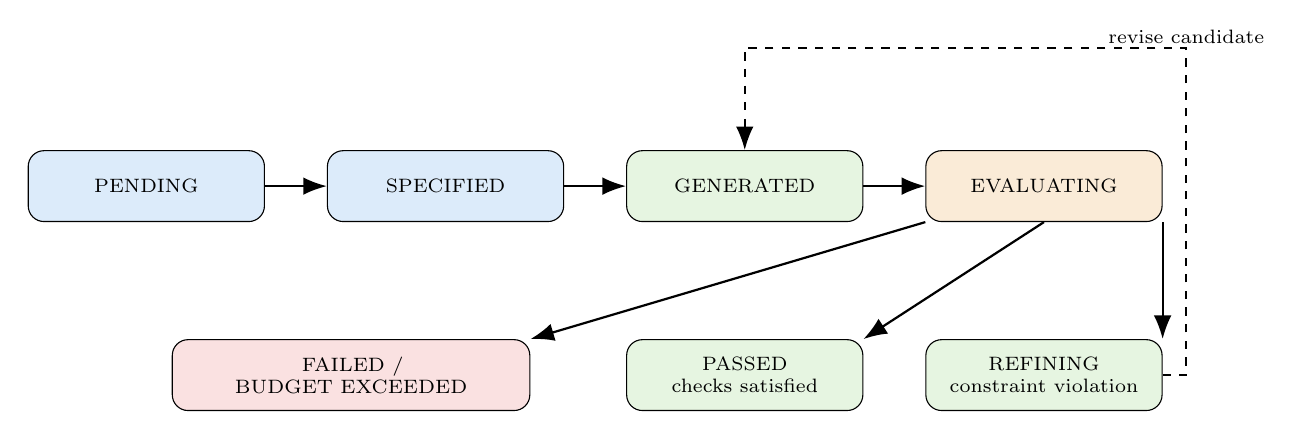
\begin{tikzpicture}[
  st/.style={rectangle,rounded corners=2mm,draw,minimum width=30mm,minimum height=9mm,align=center,inner sep=2pt,font=\scriptsize},
  failed/.style={st,text width=44mm,fill=risk},
  ar/.style={-{Latex[length=3mm]},thick}
]
\node[st,fill=architect] (pending) at (-5.7,0) {PENDING};
\node[st,fill=architect] (specified) at (-1.9,0) {SPECIFIED};
\node[st,fill=writer] (generated) at (1.9,0) {GENERATED};
\node[st,fill=evaluator] (evaluating) at (5.7,0) {EVALUATING};
\node[failed] (failed) at (-3.1,-2.4) {FAILED /\\BUDGET EXCEEDED};
\node[st,fill=writer] (passed) at (1.9,-2.4) {PASSED\\checks satisfied};
\node[st,fill=writer] (refine) at (5.7,-2.4) {REFINING\\constraint violation};

\draw[ar] (pending.east) -- (specified.west);
\draw[ar] (specified.east) -- (generated.west);
\draw[ar] (generated.east) -- (evaluating.west);
\draw[ar] (evaluating.south east) -- (refine.north east);
\draw[ar,dashed] (refine.east) -- ++(3mm,0) |- node[pos=0.5,above,font=\scriptsize,fill=white,inner sep=1pt]{revise candidate} ($(generated.north)+(0,13mm)$) -- (generated.north);
\draw[ar] (evaluating.south) -- (passed.north east);
\draw[ar] (evaluating.south west) -- (failed.north east);
\end{tikzpicture}
\caption{Core state machine.}
\end{figure}

The system should make all state transitions explicit. This is essential for replay, debugging,
benchmarking, and scientific evaluation.

The candidate loop is transactional: an artifact enters evaluation only after generation succeeds,
and it reaches \texttt{PASSED} only after validation and correctness checks both succeed. A failed
constraint returns the report to refinement with a specific diagnosis; exhausting the iteration
budget or encountering a fatal harness error terminates the run instead of permitting an unbounded
retry. The dashed return edge in the diagram represents a new candidate revision, not an in-place
mutation of the previously measured artifact.

\section{Termination Criteria}

A refinement loop terminates when:

\begin{equation}
\mathrm{Stop}(S_t)=
C_{\mathrm{pass}}
\lor
C_{\mathrm{budget}}
\lor
C_{\mathrm{stall}}
\lor
C_{\mathrm{unsafe}}.
\end{equation}

Here:

\begin{itemize}
  \item $C_{\mathrm{pass}}$ means all acceptance criteria are satisfied;
  \item $C_{\mathrm{budget}}$ means the iteration or compute budget is exhausted;
  \item $C_{\mathrm{stall}}$ means recent transformations provide no meaningful improvement;
  \item $C_{\mathrm{unsafe}}$ means execution should not continue.
\end{itemize}

\section{Transition Audit Record}

Each state change should produce an immutable event so that a failed run can be replayed without
depending on transient agent context. A transition event can be modeled as

\begin{equation}
e_t=(S_t,S_{t+1},r_t,i_t,h_{P_t},h_{R_t},H_t),
\qquad
S_{t+1}=\delta(S_t,e_t),
\end{equation}

where $r_t$ is the transition reason, $i_t$ is the refinement iteration, $h_{P_t}$ identifies
the immutable shader artifact, $h_{R_t}$ identifies its evaluation report, and $H_t$ identifies
the device and runtime profile.

The event log should retain the validation gate that allowed the transition, timestamps, and any
failure code. A retry creates a new artifact identifier rather than overwriting a previously
measured shader; this preserves the causal link between a source revision, its correctness result,
and its timing data.

\begin{longtable}{@{}>{\raggedright\arraybackslash}p{0.20\textwidth}>{\raggedright\arraybackslash}p{0.32\textwidth}>{\raggedright\arraybackslash}p{0.38\textwidth}@{}}
\toprule
\textbf{Transition} & \textbf{Guard} & \textbf{Evidence to retain}\\
\midrule
\endfirsthead
\toprule
\textbf{Transition} & \textbf{Guard} & \textbf{Evidence to retain}\\
\midrule
\endhead
Pending $\rightarrow$ specified & Request parsed; assumptions recorded & Normalized request and MathSpec identifier\\
Specified $\rightarrow$ generated & Schema and resource checks pass & Specification hash and selected configuration\\
Generated $\rightarrow$ evaluating & Static analysis and pipeline creation succeed & Artifact hash and validation report\\
Evaluating $\rightarrow$ passed & Correctness, numerical, and safety gates pass & Evaluation report and accepted metrics\\
Evaluating $\rightarrow$ refining & Recoverable issue remains; budget is available & Failure code and proposed transformation\\
Nonterminal $\rightarrow$ failed & Fatal device error or budget exhaustion & Terminal reason and last durable artifact/report\\
\bottomrule
\end{longtable}

\chapter{Hardware Capability Model}

\section{Capability Discovery}

At runtime, the harness should discover:

\begin{itemize}
  \item adapter identity,
  \item backend information when exposed,
  \item supported WebGPU features,
  \item device limits,
  \item timestamp-query support,
  \item subgroup support,
  \item subgroup-size control where supported,
  \item F16 support,
  \item relevant texture/storage format capabilities.
\end{itemize}

The 2026 WebGPU specification lists optional capabilities including timestamp queries,
\texttt{shader-f16}, subgroups, subgroup-size control, and several texture and blending features.
These must be treated as optional capabilities rather than universal assumptions.

\section{Capability Tiers}

A practical abstraction is:

\begin{description}
  \item[Tier 0] Core WebGPU functionality.
  \item[Tier 1] Profiling and timestamp capabilities.
  \item[Tier 2] Numerical acceleration such as F16.
  \item[Tier 3] Subgroup-oriented optimization.
  \item[Tier 4] Advanced format and specialized hardware capabilities.
\end{description}

A shader may have multiple variants:

\[
P =
\{P_{\mathrm{core}},
P_{\mathrm{f16}},
P_{\mathrm{subgroup}},
P_{\mathrm{hybrid}}\}.
\]

The dispatcher selects a compatible candidate at runtime.

\chapter{Safety and Isolation}

\section{Threat Model}

Generated shaders are executable programs. Although they operate within WebGPU's abstraction,
the project must assume that generated workloads can be pathological.

Threats include:

\begin{itemize}
  \item infinite or extremely long loops,
  \item enormous dispatch dimensions,
  \item excessive buffer allocations,
  \item resource exhaustion,
  \item intentionally generated invalid shaders,
  \item denial-of-service against the evaluator,
  \item driver instability,
  \item non-deterministic output,
  \item hostile host-side generated code.
\end{itemize}

\section{Execution Guardrails}

The execution harness should enforce:

\begin{align}
D &\le D_{\max},\\
B &\le B_{\max},\\
L &\le L_{\max},\\
T &\le T_{\max},
\end{align}

where $D$ is total dispatch work, $B$ is allocated buffer memory, $L$ is loop/iteration budget,
and $T$ is wall-clock execution time.

The important architectural distinction is that these are \emph{harness-level constraints}, not
source-code modifications. The system should not silently rewrite a shader in a way that changes
its semantics merely to make it safe. Instead, unsafe candidates should be rejected or executed
under explicitly documented profiling constraints.

\section{TDR and Long-Running Workloads}

The proposal should not assume that a browser-level timeout is equivalent to preventing every
possible GPU-driver failure mode. A robust design uses multiple layers:

\begin{enumerate}
  \item bounded benchmark sizes;
  \item bounded dispatch dimensions;
  \item execution watchdogs;
  \item disposable browser/device contexts;
  \item host-process supervision;
  \item benchmark cancellation;
  \item failure quarantine;
  \item automatic rollback to the last known-good artifact.
\end{enumerate}

\chapter{Reproducibility}

\section{Experiment Identity}

Each evaluation receives a unique experiment record:

\begin{equation}
E=
(
\mathrm{shaderHash},
\mathrm{mathHash},
\mathrm{hardwareHash},
\mathrm{inputHash},
\mathrm{configurationHash},
\mathrm{timestamp}
).
\end{equation}

A result is reproducible only if the important members of this tuple are preserved.

\section{Benchmark Manifest}

A benchmark manifest should contain:

\begin{itemize}
  \item workload name,
  \item input size,
  \item random seed,
  \item reference output hash,
  \item expected numerical tolerance,
  \item dispatch dimensions,
  \item feature requirements,
  \item target budget,
  \item warm-up count,
  \item measured iteration count.
\end{itemize}

\section{Warm-Up Protocol}

A robust measurement protocol is:

\[
\underbrace{W_1,\ldots,W_k}_{\text{warm-up}}
\rightarrow
\underbrace{M_1,\ldots,M_n}_{\text{measurement}}.
\]

The evaluator should record whether pipeline compilation, resource creation, and data upload are
included in the measurement.

\chapter{Repository Architecture}

The proposed repository is a monorepo separating the agent runtime from the WebGPU execution
runtime.

\begin{figure}[H]
\centering
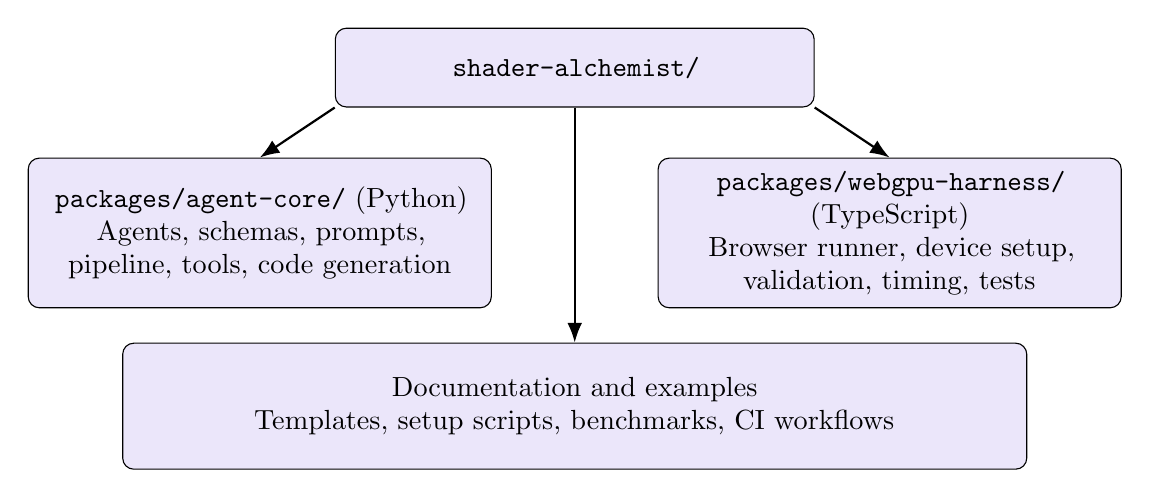
\begin{tikzpicture}[
  rootbox/.style={rectangle,rounded corners,draw,fill=infra,text width=58mm,minimum height=10mm,align=center,inner sep=4pt},
  module/.style={rectangle,rounded corners,draw,fill=infra,text width=56mm,minimum height=19mm,align=center,inner sep=4pt},
  support/.style={rectangle,rounded corners,draw,fill=infra,text width=112mm,minimum height=16mm,align=center,inner sep=4pt},
  arrow/.style={-{Latex[length=2.5mm]},thick},
]
\node[rootbox] (root) at (0,2.1) {\texttt{shader-alchemist/}};
\node[module] (agent) at (-4,0) {\texttt{packages/agent-core/} (Python)\\Agents, schemas, prompts, pipeline, tools, code generation};
\node[module] (harness) at (4,0) {\texttt{packages/webgpu-harness/} (TypeScript)\\Browser runner, device setup, validation, timing, tests};
\node[support] (support) at (0,-2.2) {Documentation and examples\\Templates, setup scripts, benchmarks, CI workflows};

\draw[arrow] (root.south west) -- (agent.north);
\draw[arrow] (root.south east) -- (harness.north);
\draw[arrow] (root.south) -- (support.north);
\end{tikzpicture}
\caption{Logical repository decomposition.}
\end{figure}

\section{Directory Specification}

\begin{lstlisting}[caption={Repository tree; documentation-oriented, not executable code.}]
shader-alchemist/
|-- .github/
|   |-- workflows/
|   |   |-- ci.yml
|   |   `-- benchmark.yml
|   `-- ISSUE_TEMPLATE/
|       `-- bug_report.md
|
|-- docs/
|   |-- architecture/
|   |   |-- system-topology.png
|   |   |-- state-machine.md
|   |   `-- memory-alignment-rules.md
|   |-- examples/
|   |   |-- spatial-hash-3d.md
|   |   `-- sph-fluid-sim.md
|   `-- api-reference.md
|
|-- packages/
|   |-- agent-core/
|   |   |-- pyproject.toml
|   |   |-- README.md
|   |   `-- src/shader_alchemist/
|   |       |-- __init__.py
|   |       |-- main.py
|   |       |-- config.py
|   |       |-- agents/
|   |       |   |-- __init__.py
|   |       |   |-- math_architect.py
|   |       |   |-- wgsl_writer.py
|   |       |   |-- evaluator.py
|   |       |   `-- prompts/
|   |       |       |-- math_architect.jinja2
|   |       |       |-- wgsl_writer.jinja2
|   |       |       `-- evaluator.jinja2
|   |       |-- schemas/
|   |       |   |-- __init__.py
|   |       |   |-- state.py
|   |       |   |-- math_spec.py
|   |       |   |-- artifact.py
|   |       |   `-- eval_report.py
|   |       |-- pipeline/
|   |       |   |-- __init__.py
|   |       |   |-- sequential.py
|   |       |   |-- loop_block.py
|   |       |   `-- state_manager.py
|   |       |-- tools/
|   |       |   |-- __init__.py
|   |       |   |-- profiler_tool.py
|   |       |   `-- static_analyzer.py
|   |       `-- codegen/
|   |           |-- __init__.py
|   |           |-- ts_driver_generator.py
|   |           `-- report_generator.py
|   |   |-- tests/
|   |   |   |-- test_math_architect.py
|   |   |   |-- test_wgsl_writer.py
|   |   |   `-- test_pipeline_loop.py
|
|   `-- webgpu-harness/
|       |-- package.json
|       |-- tsconfig.json
|       |-- README.md
|       |-- src/
|       |   |-- index.ts
|       |   |-- browser-runner.ts
|       |   |-- profiler/
|       |   |   |-- device.ts
|       |   |   |-- buffer-allocator.ts
|       |   |   |-- query-set.ts
|       |   |   `-- validation-scope.ts
|       |   |-- templates/runner-page.html
|       |   `-- utils/time.ts
|       `-- tests/
|           |-- harness.test.ts
|           `-- timestamp-query.test.ts
|
|-- templates/
|   |-- typescript/
|   |   |-- package.json.jinja2
|   |   |-- tsconfig.json.jinja2
|   |   `-- webgpu_app.ts.jinja2
|   `-- html/standalone_demo.html.jinja2
|
|-- scripts/
|   |-- setup_environment.sh
|   |-- run_harness_server.sh
|   `-- benchmark_all_examples.py
|
|-- .gitignore
|-- .env.example
|-- pnpm-workspace.yaml
|-- README.md
|-- LICENSE
`-- project configuration
\end{lstlisting}

The tree separates the Python reasoning and orchestration runtime from the TypeScript execution
runtime. Within \texttt{agent-core}, the three agent modules own bounded responsibilities:
\texttt{math\_architect.py} creates the formal contract, \texttt{wgsl\_writer.py} emits shader
candidates from that contract, and \texttt{evaluator.py} interprets harness evidence and proposes
diagnoses. Their prompts are kept separately from orchestration code so behavior can be versioned
and tested independently. The \texttt{schemas/} package defines the state, specification,
artifact, and report contracts shared across stages; \texttt{pipeline/} manages stage ordering,
refinement limits, and state transitions.

The \texttt{tools/} package is the boundary to external validation and measurement. In particular,
\texttt{profiler\_tool.py} acts as a narrow bridge to the harness rather than embedding browser
execution in the agent process. The TypeScript package owns device discovery, buffer allocation,
validation scopes, timing queries, and the browser runner. Its CLI or IPC response should use a
versioned structured message so a Python-side schema can reject incomplete or incompatible
reports. Templates and code generators package the selected artifact for users; they do not
change the correctness contract established earlier in the pipeline.

The CI workflow should test schema and agent behavior separately from harness behavior. Benchmark
automation should retain device, browser, driver, feature, and measurement-mode metadata with every
run; results from unlike environments must not be treated as a direct regression comparison. The
directory names describe intended component boundaries, not a requirement to implement every
subsystem in the first milestone.

\chapter{Data Contracts}

\section{MathSpec}

Conceptually:

\begin{equation}
\MathSpec =
(
A,D,L,B,S,N,H,V
).
\end{equation}

\begin{longtable}{p{0.22\textwidth}p{0.30\textwidth}p{0.38\textwidth}}
\toprule
\textbf{Field} & \textbf{Meaning} & \textbf{Purpose}\\
\midrule
Algorithm & Algorithm identity & Semantic traceability\\
Domain & Input/output mathematical domain & Correctness reasoning\\
Workgroups & Candidate dimensions & Parallel decomposition\\
Dispatch & Derived dispatch geometry & Execution correctness\\
Buffers & Host-shareable layouts & Memory compatibility\\
Bindings & Resource contracts & Pipeline validation\\
Synchronization & Barriers / atomics / pass boundaries & Race prevention\\
Numerics & Precision and tolerances & Numerical verification\\
Capabilities & Required optional features & Portability\\
Invariants & Properties that must hold & Automated testing\\
\bottomrule
\end{longtable}

The following compact instance makes the contract concrete for a 1025-element vector addition.
It is illustrative serialization rather than a required final schema; in an implementation,
Pydantic validation should reject missing bindings, unsupported features, and dispatch dimensions
that disagree with the element count and workgroup shape.

\begin{lstlisting}[caption={Illustrative MathSpec instance for vector addition.}]
{
  "schema_version": 1,
  "algorithm": "vector_add",
  "entry_point": "vector_add",
  "domain": {"element_count": 1025},
  "workgroup_size": [64, 1, 1],
  "dispatch": [17, 1, 1],
  "bindings": [
    {"group": 0, "binding": 0, "name": "lhs", "access": "read", "element_type": "f32"},
    {"group": 0, "binding": 1, "name": "rhs", "access": "read", "element_type": "f32"},
    {"group": 0, "binding": 2, "name": "output_buffer", "access": "read_write", "element_type": "f32"}
  ],
  "numerics": {"atol": 1e-6, "rtol": 1e-5},
  "required_features": [],
  "invariants": ["input_lengths_equal", "output_length_equals_input_length"]
}
\end{lstlisting}

Dispatch is derived from the domain and workgroup size, so the serialized values are checked
rather than trusted as independent inputs. The same principle applies to byte lengths, binding
limits, and optional capabilities: store the requested configuration, then verify it against the
actual device profile before pipeline creation.

\section{ShaderArtifact}

The artifact is more than WGSL source:

\begin{equation}
\ShaderArtifact=
(
S,
E,
B,
D,
F,
G
),
\end{equation}

where $S$ is source, $E$ entry points, $B$ binding metadata, $D$ dispatch information,
$F$ feature requirements, and $G$ provenance metadata.

\section{EvalReport}

\begin{equation}
\EvalReport=
(
V,
T,
C,
M,
N,
O,
R
),
\end{equation}

where:

\begin{itemize}
  \item $V$ = validation result,
  \item $T$ = timing measurements,
  \item $C$ = correctness results,
  \item $M$ = memory/resource observations,
  \item $N$ = numerical errors,
  \item $O$ = optimization observations,
  \item $R$ = remediation recommendations.
\end{itemize}

\chapter{Observability and Telemetry}

\section{Why Observability Matters}

Agentic optimization is difficult to debug without a detailed trace. The system therefore records
the causal history:

\[
\text{request}
\rightarrow
\text{MathSpec}
\rightarrow
\text{transformation}
\rightarrow
\text{artifact}
\rightarrow
\text{measurement}
\rightarrow
\text{decision}.
\]

Every optimization should have provenance.

\section{Optimization Provenance}

For transformation $\tau_i$:

\begin{equation}
\tau_i=
(
\mathrm{name},
\mathrm{reason},
\mathrm{preconditions},
\mathrm{beforeHash},
\mathrm{afterHash},
\mathrm{expectedEffect},
\mathrm{measuredEffect}
).
\end{equation}

This permits later analysis of which transformations actually work.

\chapter{Evaluation Methodology}

\section{Baseline Comparisons}

The system should be evaluated against at least four baselines:

\begin{enumerate}
  \item direct language-model shader generation;
  \item rule-based shader generation without iterative evaluation;
  \item generated shader plus static validation;
  \item full \SA{} closed-loop system.
\end{enumerate}

The goal is not simply to show that the complete system works, but to identify which architectural
components provide measurable value.

\section{Ablation Studies}

Potential ablations include:

\begin{itemize}
  \item remove Math Architect;
  \item remove performance feedback;
  \item remove static layout analysis;
  \item remove reference-output verification;
  \item remove hardware capability profiling;
  \item remove optimization history;
  \item remove transformation registry.
\end{itemize}

For each ablation, measure:

\begin{align}
\text{Validity Rate} &= \frac{\text{valid candidates}}{\text{all candidates}},\\
\text{Correctness Rate} &= \frac{\text{correct candidates}}{\text{valid candidates}},\\
\text{Median Speedup} &= \operatorname{median}\left(\frac{T_{\mathrm{baseline}}}{T_{\mathrm{candidate}}}\right),\\
\text{Search Cost} &= \text{GPU executions per accepted candidate}.
\end{align}

\section{Research Benchmark Matrix}

\begin{longtable}{p{0.20\textwidth}p{0.20\textwidth}p{0.23\textwidth}p{0.25\textwidth}}
\toprule
\textbf{Workload} & \textbf{Dominant Cost} & \textbf{Optimization} & \textbf{Correctness Criterion}\\
\midrule
Spatial hashing & Atomics / memory & Layout, bucket strategy & Neighbor-set equivalence\\
Particle integration & Arithmetic & Workgroup tuning & Numerical tolerance\\
Reduction & Synchronization & Subgroups / shared memory & Exact or bounded error\\
Image convolution & Bandwidth & Tiling / cache reuse & Pixel error bound\\
Matrix kernel & Compute / bandwidth & Tiling / precision & Relative error\\
Prefix operation & Dependencies & Multi-stage decomposition & Sequence equivalence\\
\bottomrule
\end{longtable}

\chapter{Advanced Capabilities}

\section{Subgroup-Aware Optimization}

When subgroup operations are available, reductions can potentially be expressed with fewer shared
memory operations.

A reduction over values $x_0,\ldots,x_{N-1}$ computes

\begin{equation}
R=\bigoplus_{i=0}^{N-1}x_i.
\end{equation}

A hierarchical design may be:

\[
\text{invocation}
\rightarrow
\text{subgroup reduction}
\rightarrow
\text{workgroup reduction}
\rightarrow
\text{global reduction}.
\]

The optimizer should only select this path when capability discovery confirms support and the
algorithm's numerical and semantic requirements permit it.

\section{F16 and Mixed Precision}

For suitable workloads, the optimizer can model precision as a resource:

\[
P\in\{\mathrm{f32},\mathrm{f16},\mathrm{mixed}\}.
\]

A mixed-precision algorithm may compute intermediate values in lower precision while retaining
accumulation or critical state in higher precision.

The acceptance condition becomes:

\begin{equation}
E(P)\le\epsilon
\end{equation}

rather than simply assuming that lower precision is acceptable.

\section{Autotuning}

Suppose the candidate parameter vector is

\[
\theta=(W_x,W_y,W_z,T,B,S,\ldots).
\]

The optimizer evaluates

\[
f(\theta)=T(P_\theta).
\]

A naive grid search costs

\[
O\left(\prod_i |\Theta_i|\right).
\]

This can become expensive rapidly. Bayesian optimization or successive-halving strategies can
reduce the number of expensive GPU measurements.

\section{Learned Performance Model}

With historical data

\[
\mathcal{D}
=
\{(x_i,\theta_i,T_i)\}_{i=1}^{N},
\]

a model can estimate

\[
\hat{T}=f_\phi(x,\theta,H).
\]

The learned model should be treated as a search heuristic, not as a replacement for actual
measurement. The evaluator remains the authority for final performance claims.

\section{Counterfactual Optimization}

An especially powerful future feature is counterfactual reasoning:

\[
P
\rightarrow
\{\tau_1(P),\tau_2(P),\ldots,\tau_k(P)\}.
\]

Instead of making one optimization and hoping it works, the system generates a small beam of
candidate transformations and empirically tests them.

This converts the loop into a controlled experiment:

\[
\boxed{
\text{Generate hypotheses}
\rightarrow
\text{Measure}
\rightarrow
\text{Rank by evidence}
\rightarrow
\text{Expand promising branches}
}
\]

The approach resembles beam search over program transformations, with GPU measurements serving
as the objective function.

\chapter{Visual Verification}

\section{Motivation}

Many compute shaders ultimately produce images or spatial fields. Numerical validation alone may
miss perceptual artifacts.

A visual verification subsystem can render:

\[
I_{\mathrm{candidate}},\qquad I_{\mathrm{reference}}.
\]

Pixel error can be defined as:

\begin{equation}
E_{\mathrm{pixel}}
=
\frac{1}{N}
\sum_{p=1}^{N}
\|I_c(p)-I_r(p)\|_2.
\end{equation}

Structural similarity, perceptual metrics, edge differences, and temporal consistency can be
added for visual workloads.

The visual evaluator should be supplementary rather than authoritative for scientific workloads.

\chapter{Multi-Pass Pipeline Synthesis}

\section{Why Multi-Pass Matters}

Many algorithms cannot be safely expressed as a single compute pass because global dependencies
exist between workgroups.

The system therefore treats a complete computation as a graph:

\[
\mathcal{P}
=
(P_1,P_2,\ldots,P_k),
\]

where each pass has:

\[
P_i=(S_i,B_i,D_i,O_i).
\]

A dependency edge

\[
P_i\rightarrow P_j
\]

means that the output of $P_i$ is required by $P_j$.

\section{SPH Case Study and Pass Contracts}

Smoothed particle hydrodynamics (SPH) illustrates why the mathematical model, spatial index, and
pass graph must be designed together. For particle $i$, let $\mathcal{N}(i)$ contain candidate
neighbors within the compact support radius of a smoothing kernel $W_h$. A simplified density
estimate is

\begin{equation}
\rho_i=\sum_{j\in\mathcal{N}(i)}m_j
W_h\!\left(\|\mathbf{x}_i-\mathbf{x}_j\|\right),
\qquad
p_i=c_s^2(\rho_i-\rho_0),
\end{equation}

where $m_j$ is particle mass, $h$ is the smoothing length, $c_s$ is a model parameter, and
$\rho_0$ is the reference density. A symmetric pressure-force term is

\begin{equation}
\mathbf{a}_i^{\mathrm{pressure}}
=-\sum_{j\in\mathcal{N}(i)}m_j
\left(\frac{p_i}{\rho_i^2}+\frac{p_j}{\rho_j^2}\right)
\nabla_i W_h\!\left(\|\mathbf{x}_i-\mathbf{x}_j\|\right).
\end{equation}

With an external acceleration $\mathbf{g}$, a simple semi-implicit Euler update is

\begin{align}
\mathbf{v}_i^{n+1}&=\mathbf{v}_i^n+\Delta t
\left(\mathbf{a}_i^{\mathrm{pressure}}+\mathbf{g}\right),\\
\mathbf{x}_i^{n+1}&=\mathbf{x}_i^n+\Delta t\,\mathbf{v}_i^{n+1}.
\end{align}

This simplified model omits viscosity, boundary forces, and adaptive time stepping; those terms
must be added to the specification when required by the intended simulation. The dependency graph
for one time step is nevertheless explicit:

\begin{lstlisting}[caption={Conceptual pass sequence for one SPH time step.}]
clear cell counts
build spatial index from current positions
compute particle densities and pressures
compute accelerations from neighboring particles
integrate into next-position and next-velocity buffers
swap current and next state buffers
\end{lstlisting}

The spatial-index pass must finish before density evaluation; density and pressure must finish
before force evaluation; and all force reads must finish before state is advanced. Separate
dispatches provide these global phase boundaries. Ping-pong state buffers avoid races between
invocations that read neighboring particles and invocations that write updated state. If the
average number of candidate neighbors is $\bar{k}$, a well-behaved spatial index reduces expected
neighbor work from $O(N^2)$ to approximately $O(N\bar{k})$, while dense cells and hash collisions
can still increase the actual cost.

\section{Pipeline-Level Optimization}

The optimizer can now trade:

\begin{itemize}
  \item fewer dispatches,
  \item more local work,
  \item more memory traffic,
  \item more synchronization,
  \item greater algorithmic complexity.
\end{itemize}

The objective becomes:

\begin{equation}
T_{\mathrm{pipeline}}
=
\sum_i T(P_i)
+
\sum_i T_{\mathrm{boundary},i}.
\end{equation}

This is more realistic than optimizing each kernel independently.

\chapter{Compiler and Toolchain Integration}

\section{Static Validation}

The system should support compiler-backed validation through appropriate WGSL tooling. A static
analysis layer can detect:

\begin{itemize}
  \item parse errors,
  \item type errors,
  \item invalid resource declarations,
  \item impossible binding layouts,
  \item unsupported feature assumptions,
  \item suspicious memory accesses,
  \item uniformity hazards where detectable.
\end{itemize}

Static analysis is a filter, not a proof of runtime correctness.

\section{Cross-Representation Validation}

A future architecture can use multiple representations:

\[
\text{MathSpec}
\rightarrow
\text{Shader IR}
\rightarrow
\text{WGSL}
\rightarrow
\text{backend representation}.
\]

Cross-checking multiple representations creates opportunities for stronger diagnostics.

\chapter{Future Cross-API Architecture}

Although WebGPU is the primary target, the internal architecture can be made backend-neutral.

\begin{figure}[H]
\centering
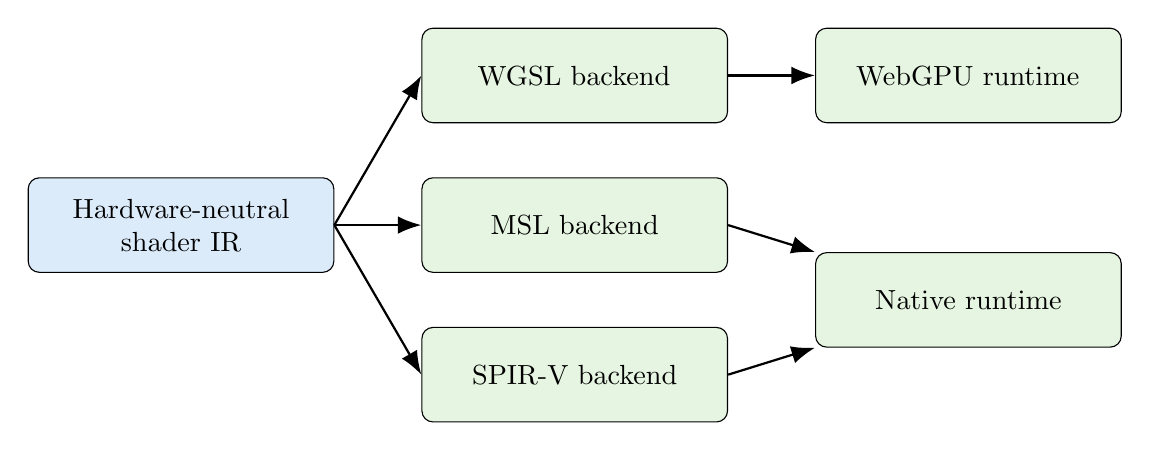
\begin{tikzpicture}[
  n/.style={rectangle,rounded corners,draw,text width=36mm,minimum height=12mm,align=center,inner sep=4pt},
  a/.style={-{Latex[length=3mm]},thick}
]
\node[n,fill=architect] (ir) at (0,0) {Hardware-neutral\\shader IR};
\node[n,fill=writer] (wgsl) at (5,1.9) {WGSL backend};
\node[n,fill=writer] (msl) at (5,0) {MSL backend};
\node[n,fill=writer] (spirv) at (5,-1.9) {SPIR-V backend};
\node[n,fill=writer] (webgpu) at (10,1.9) {WebGPU runtime};
\node[n,fill=writer] (native) at (10,-0.95) {Native runtime};
\draw[a] (ir.east) -- (wgsl.west);
\draw[a] (ir.east) -- (msl.west);
\draw[a] (ir.east) -- (spirv.west);
\draw[a] (wgsl.east) -- (webgpu.west);
\draw[a] (msl.east) -- (native.north west);
\draw[a] (spirv.east) -- (native.south west);
\end{tikzpicture}
\caption{Potential future cross-API architecture.}
\end{figure}

The mathematical specification therefore becomes the stable semantic layer, while individual
backends become code-generation and evaluation targets.

The shared layer should describe operation semantics, logical types, resource intent, synchronization
requirements, and numerical policy without assuming one API's binding syntax. A backend then lowers
that contract into its own shader language and pipeline layout; a runtime adapter handles device
discovery, resource creation, execution, and measurement. These boundaries are important because
similar-looking GPU APIs can differ in memory layout, optional features, synchronization, and
timing support.

Every backend should run the same reference workloads and correctness properties before its
performance results are compared. Unsupported operations should produce an explicit capability
failure or a verified fallback, not a silently weakened implementation. Cross-API portability is
therefore a tested property of each artifact and device profile, not an assumption made from the
existence of a common intermediate representation.

\chapter{Agent Memory and Learning}

\section{Optimization Memory}

The system should maintain a structured optimization memory:

\[
\mathcal{H}
=
\{
(\text{workload},\text{hardware},\text{transformation},\Delta T)
\}.
\]

For a new workload, similar historical cases can suggest promising transformations.

\section{Memory Should Store Evidence, Not Just Text}

A useful memory record contains:

\begin{itemize}
  \item workload fingerprint,
  \item hardware fingerprint,
  \item transformation,
  \item preconditions,
  \item measured result,
  \item confidence,
  \item correctness result,
  \item failure modes.
\end{itemize}

This prevents the agent from learning the simplistic rule ``tiling is good'' and instead learns
conditional rules such as ``tiling improved bandwidth-bound convolution under this class of
workloads and resource constraints.''

\chapter{Human-in-the-Loop Mode}

Automation should not eliminate expert control. The system should provide modes such as:

\begin{description}
  \item[Explain] Generate a mathematically detailed explanation without execution.
  \item[Validate] Validate a user-provided shader.
  \item[Optimize] Search for faster variants while preserving semantics.
  \item[Explore] Generate multiple algorithmic strategies.
  \item[Benchmark] Compare explicitly supplied implementations.
  \item[Research] Run a reproducible experiment suite.
\end{description}

For advanced users, the interface can expose the optimization frontier rather than hiding the
search behind a single answer.

\chapter{Failure Taxonomy}

A major research value of \SA{} is the ability to classify failures.

\begin{longtable}{p{0.21\textwidth}p{0.31\textwidth}p{0.34\textwidth}}
\toprule
\textbf{Failure Class} & \textbf{Example} & \textbf{Preferred Response}\\
\midrule
Semantic & Wrong algorithm & Rebuild MathSpec\\
Type / compile & Invalid WGSL type & Repair artifact\\
Layout & Host/shader mismatch & Recompute layout\\
Resource & Binding mismatch & Reconcile pipeline contract\\
Race & Concurrent unsafe write & Atomic or multi-pass redesign\\
Numerical & Excessive floating error & Precision redesign\\
Performance & Kernel too slow & Transformation search\\
Portability & Optional feature unavailable & Select fallback variant\\
Harness & Browser/GPU unavailable & Change execution mode\\
Stall & No improvement after several iterations & Terminate / escalate\\
\bottomrule
\end{longtable}

This taxonomy should become a dataset for future agent training and evaluation.

\chapter{Example End-to-End Scenario}

Consider the request:

\begin{quote}
``Build a compute pipeline for a 3D particle system using spatial hashing so that neighboring
particles can be queried efficiently.''
\end{quote}

The system performs the following reasoning:

\begin{enumerate}
  \item Identify particles as the primary parallel domain.
  \item Define spatial cells using cell width $s$.
  \item Derive integer cell coordinates.
  \item Construct a hash representation.
  \item Determine bucket representation.
  \item Determine insertion semantics.
  \item Identify collision and contention behavior.
  \item Determine whether neighbor traversal requires one or multiple passes.
  \item Generate a candidate layout.
  \item Generate a candidate WGSL implementation.
  \item Validate the pipeline.
  \item Run correctness tests against a CPU reference.
  \item Benchmark several workgroup configurations.
  \item Compare alternative data layouts.
  \item Record the winning candidates and rejected hypotheses.
\end{enumerate}

The final result is not merely shader text. It is an evidence package:

\[
\boxed{
\begin{gathered}
\text{Shader}+\text{Mathematical Contract}+\text{Host Layout}\\
+\text{Correctness Evidence}+\text{Performance Evidence}\\
+\text{Provenance}
\end{gathered}
}
\]

\chapter{Deployment Architecture}

\section{Local Development}

A local developer installation can use:

\[
\text{CLI}
\rightarrow
\text{Agent Runtime}
\rightarrow
\text{Local Harness}
\rightarrow
\text{Local GPU}.
\]

This mode maximizes privacy and minimizes network latency.

\section{Remote Evaluation}

A research server can expose:

\[
\text{Agent}
\rightarrow
\text{Job Queue}
\rightarrow
\text{GPU Worker}
\rightarrow
\text{Result Store}.
\]

A worker should be treated as ephemeral:

\[
\text{provision}
\rightarrow
\text{execute}
\rightarrow
\text{collect}
\rightarrow
\text{destroy}.
\]

This is particularly useful for benchmark farms containing different GPU architectures.

\chapter{Benchmark Farm}

A mature version can maintain hardware-specific workers:

\[
H_1,H_2,\ldots,H_n.
\]

For each candidate $P$:

\[
\mathbf{T}(P)=
[T(P,H_1),T(P,H_2),\ldots,T(P,H_n)].
\]

This enables analysis of portability.

A candidate that is fast on one architecture but poor on every other device is fundamentally
different from a candidate with consistent performance.

The system can therefore report:

\begin{equation}
\mu_H(P)=\operatorname{mean}_j T(P,H_j)
\end{equation}

and

\begin{equation}
\sigma_H(P)=\operatorname{std}_j T(P,H_j).
\end{equation}

These are not substitutes for device-specific measurements, but they provide a useful robustness
signal.

\chapter{Scientific Contribution}

The project has the potential to contribute beyond a developer tool.

\section{Contribution 1: Agentic GPU Compilation}

It explores a compiler pipeline where an LLM-based agent operates at the semantic and optimization
layers while deterministic tools establish execution evidence.

\section{Contribution 2: Closed-Loop Shader Synthesis}

The central loop,

\[
\text{generate}\rightarrow\text{execute}\rightarrow\text{measure}\rightarrow\text{refine},
\]

provides a concrete framework for studying empirical program synthesis on GPUs.

\section{Contribution 3: Evidence-Centric Agent State}

The state contains not only generated text but also:

\[
\text{hypotheses}+\text{measurements}+\text{failures}+\text{transformations}.
\]

This makes the agent's optimization process auditable.

\section{Contribution 4: Hardware-Conditional Program Generation}

Instead of generating one universal shader, the system generates a conditional family:

\[
\mathcal{P}(H)=\{P_1,P_2,\ldots,P_k\}.
\]

The runtime then selects an appropriate implementation.

\chapter{Limitations}

The proposal has important limitations.

\begin{enumerate}
  \item GPU timing remains implementation-dependent and can contain noise.
  \item Browser and driver behavior can vary between systems.
  \item Some performance characteristics are difficult to observe through WebGPU.
  \item Agent-generated optimizations can accidentally alter semantics.
  \item Hardware-specific tuning can reduce portability.
  \item Large optimization spaces can become prohibitively expensive.
  \item A benchmark result is not automatically a universal performance claim.
  \item Numerical equivalence can be difficult for chaotic simulations.
  \item Security isolation around GPU execution requires careful engineering.
\end{enumerate}

These limitations are not reasons to avoid the system. They define the experimental boundaries
within which its claims should be made.

\chapter{Development Roadmap}

\begin{figure}[H]
\centering
\begin{ganttchart}[
  hgrid,
  vgrid,
  x unit=0.50cm,
  y unit chart=0.42cm,
  title label font=\scriptsize\bfseries,
  bar label font=\small,
  milestone label font=\small
]{1}{18}
\gantttitle{Development Roadmap}{18}\\
\gantttitlelist{1,...,18}{1}\\
\ganttbar{Repository + schemas}{1}{2}\\
\ganttbar{Math Architect}{2}{4}\\
\ganttbar{WGSL generation layer}{3}{5}\\
\ganttbar{WebGPU harness}{4}{7}\\
\ganttbar{Validation + correctness}{6}{8}\\
\ganttbar{Closed-loop optimization}{8}{11}\\
\ganttbar{Benchmark suite}{9}{12}\\
\ganttbar{Autotuning}{11}{14}\\
\ganttbar{Capability-aware variants}{12}{15}\\
\ganttbar{Research evaluation}{14}{17}\\
\ganttbar{Documentation + release}{16}{18}
\end{ganttchart}
\caption{Illustrative development roadmap.}
\end{figure}

\paragraph*{Phase I: Deterministic Foundation} Build schemas, benchmark manifests, artifact
contracts, and a minimal harness with repeatable inputs and CPU reference outputs.

\paragraph*{Phase II: Agentic Synthesis} Add the Math Architect and WGSL Writer while keeping
the evaluator deterministic; validate each handoff against the shared data contracts.

\paragraph*{Phase III: Closed-Loop Optimization} Introduce named feedback-driven transformations,
correctness gates, and a bounded refinement budget.

\paragraph*{Phase IV: Hardware-Aware Search} Add capability profiles, parameter sweeps, fallback
variants, and benchmark history scoped to comparable devices.

\paragraph*{Phase V: Research Platform} Run replicated cross-device experiments and compare the
closed-loop system against direct shader generation. Retain manifests, failure categories,
confidence estimates, and candidate provenance so performance priors and publication claims can
be reproduced independently.

\chapter{Proposed Final Output Contract}

For each successful task, \SA{} should produce:

\begin{enumerate}
  \item final shader artifact;
  \item mathematical specification;
  \item resource and layout specification;
  \item dispatch configuration;
  \item correctness report;
  \item performance report;
  \item hardware capability profile;
  \item optimization history;
  \item rejected candidate summary;
  \item reproducibility manifest.
\end{enumerate}

A conceptual package is:

\begin{lstlisting}[caption={Illustrative output package.}]
ShaderAlchemistOutput/
|-- shader.wgsl
|-- host_driver.ts
|-- math_spec.json
|-- layout_spec.json
|-- capability_profile.json
|-- correctness_report.md
|-- performance_report.md
|-- optimization_history.json
`-- reproducibility_manifest.json
\end{lstlisting}

These are artifact names rather than production implementation requirements. The exact serialization
format may evolve.

\chapter{Conclusion}

\SA{} is best understood not as an ``AI that writes shaders'' but as an agentic GPU engineering
system.

Its fundamental abstraction is a controlled scientific loop:

\[
\boxed{
\begin{gathered}
\text{Intent}\rightarrow\text{Mathematical Model}\rightarrow\text{Parallel Specification}\\
\rightarrow\text{Shader}\rightarrow\text{Execution}\rightarrow\text{Evidence}\rightarrow\text{Optimization}
\end{gathered}
}
\]

The architecture separates reasoning from execution. The Math Architect establishes what the
algorithm means. The WGSL Writer determines how that meaning can be represented as a GPU program.
The Performance Evaluator establishes what actually happens when that program executes. The
orchestrator then decides whether the evidence justifies acceptance, revision, or abandonment.

This distinction is the central scientific idea of the project.

A language model can propose an optimization. It cannot, by reasoning alone, guarantee that the
optimization improves a particular GPU workload. Conversely, a benchmark can show that an
implementation is fast, but it cannot by itself establish that the implementation preserves the
algorithm's semantics. \SA{} therefore combines both sides:

\[
\begin{gathered}
\text{reasoning}+\text{formal contracts}\\
+\text{deterministic validation}+\text{empirical GPU measurement}.
\end{gathered}
\]

The future version of the system can grow from a three-agent prototype into a compiler-like
research platform containing a shader IR, transformation registry, hardware capability database,
benchmark farm, learned performance model, multi-pass pipeline optimizer, and cross-backend
code-generation layer.

The long-term vision is a system in which a developer can state:

\begin{quote}
``I need this computation to behave according to these equations, operate on this data domain,
respect this numerical tolerance, and meet this performance budget on these classes of hardware.''
\end{quote}

and receive not merely generated source code, but an experimentally verified implementation
together with the mathematical assumptions, execution contract, measurements, optimization
history, and evidence supporting the result.

That is the purpose of \SA{}: to turn shader generation from a text-generation problem into an
engineering discipline.

\appendix

\chapter{Glossary}

\begin{description}
  \item[Agent] A software component that performs a bounded reasoning or tool-using role.
  \item[MathSpec] Formal mathematical and execution specification produced before shader synthesis.
  \item[ShaderArtifact] A generated shader plus all metadata required to execute it.
  \item[EvalReport] Structured evidence produced by the execution and validation harness.
  \item[Workgroup] A group of compute invocations that can cooperate through workgroup-scoped
        mechanisms.
  \item[Dispatch] A command that launches compute workgroups.
  \item[Subgroup] A hardware-oriented collective execution group exposed by optional WebGPU
        capabilities when supported.
  \item[Autotuning] Empirical search over implementation parameters.
  \item[Provenance] Metadata describing how an artifact was produced and transformed.
  \item[Reference implementation] A trusted baseline used for correctness comparison.
\end{description}

\chapter{Key Equations Summary}

\begin{align}
\text{1D dispatch:}\quad
G &= \left\lceil\frac{N}{W}\right\rceil,\\[0.4em]
\text{Dispatch utilization:}\quad
\eta_{\mathrm{dispatch}} &= \frac{N}{GW},\\[0.4em]
\text{3D dispatch:}\quad
G_d &= \left\lceil\frac{N_d}{W_d}\right\rceil,\quad d\in\{x,y,z\},\\[0.4em]
\text{Spatial cell:}\quad
\mathbf{c} &= \left\lfloor\frac{\mathbf{p}-\mathbf{o}}{s}\right\rfloor,\\[0.4em]
\text{Hash:}\quad
h(\mathbf{c}) &=
(c_xP_x\oplus c_yP_y\oplus c_zP_z)\bmod B,\\[0.4em]
\text{Expected colliding pairs:}\quad
\mathbb{E}[C] &= \frac{N(N-1)}{2B},\\[0.4em]
\text{Relative error:}\quad
E_{\mathrm{rel}} &=
\frac{\|Y_g-Y_r\|_2}
{\max(\|Y_r\|_2,\epsilon)},\\[0.4em]
\text{Mixed tolerance:}\quad
|y_{g,i}-y_{r,i}| &\le \varepsilon_{\mathrm{abs}}+
\varepsilon_{\mathrm{rel}}|y_{r,i}|,\\[0.4em]
\text{Arithmetic intensity:}\quad
I &= \frac{F}{Q},\\[0.4em]
\text{Idealized roofline bound:}\quad
T &\ge \max\left(\frac{F}{\Pi_{\max}},\frac{Q}{\beta_{\max}}\right),\\[0.4em]
\text{GPU duration:}\quad
T_{\mathrm{gpu}} &= t_e-t_s,\\[0.4em]
\text{Optimization objective:}\quad
J(P) &=
\sum_i w_i f_i(P),\\[0.4em]
\text{Search transition:}\quad
P_{i+1} &= \tau_i(P_i).
\end{align}

\chapter{Reference Notes}

This proposal is aligned with the WebGPU and WGSL specifications current in 2026. In particular,
the WebGPU specification treats many capabilities as optional and explicitly includes facilities
such as \texttt{timestamp-query}, \texttt{shader-f16}, subgroups, and subgroup-size control.
The WGSL specification defines host-shareable types and address-space-specific memory layout and
memory-model rules. These details should be treated as normative constraints by the eventual
implementation rather than approximated by generic ``GPU alignment'' heuristics.

The architecture also follows the general philosophy of modern agent-development workflows:
separate agents by responsibility, represent intermediate state explicitly, make tool execution
observable, and evaluate agent behavior with reproducible workflows.

\begin{thebibliography}{9}

\bibitem{webgpu2026}
W3C GPU for the Web Working Group,
\emph{WebGPU Candidate Recommendation Draft},
15 September 2026.
\url{https://www.w3.org/TR/webgpu/}

\bibitem{wgsl2026}
W3C GPU for the Web Working Group,
\emph{WebGPU Shading Language Candidate Recommendation Draft},
September 2026.
\url{https://www.w3.org/TR/WGSL/}

\bibitem{wgslgpuweb}
GPU for the Web Community Group,
\emph{WebGPU Shading Language: Internal Layout and Memory Model}.
\url{https://gpuweb.github.io/gpuweb/wgsl/}

\bibitem{adk}
Google,
\emph{Agent Development and Agents CLI Documentation}.
\url{https://google.github.io/agents-cli/}

\end{thebibliography}

\end{document}
